\documentclass[11pt]{beamer}
\mode<presentation>
\usetheme{Hannover} % Beamer Theme
\usecolortheme{lily} % Beamer Color Theme
\newcommand{\N}{\mathbb{N}}
\newcommand{\R}{\mathbb{R}}
\newcommand{\C}{\mathbb{C}}
\newcommand{\Z}{\mathbb{Z}}
\newcommand{\Proj}{\mathbb{P}}
\newcommand{\T}{\mathbb{T}}
\newcommand{\face}{\prec}
\newcommand{\V}{\vee}
\newcommand{\m}{\mathfrak{m}}
\DeclareMathOperator{\End}{End}
\DeclareMathOperator{\Hom}{Hom}
\DeclareMathOperator{\im}{im}
\DeclareMathOperator{\Cone}{Cone}
\DeclareMathOperator{\Spec}{Spec}
\useinnertheme{rectangles}

\usepackage{amsmath}
\usepackage{graphicx}

\title{Examples}
\author{Ragib Zaman}
\institute{AMSSC at the University of Newcastle}
\date{2 July 2014}
\usepackage{amsmath,amsthm}
\usepackage{tikz}
\usetikzlibrary{calc}

\begin{document}
\begin{frame}
\titlepage
\end{frame}

\begin{frame}
\begin{Example} Take $\sigma=\Cone(e_1, e_2).$
\begin{figure}[ht]
  \centering
  \begin{tikzpicture}
    \draw [thin, gray,-latex] (-2,0) -- (3,0);% Draw x axis
    \draw [thin, gray,-latex] (0,-2) -- (0,3);% Draw y axis
    \clip (-2.05,-2.05) rectangle (3.05cm,3.05cm); 
    \draw[style=help lines,dashed] (-4,-4) grid[step=1cm] (4,4);
    \foreach \x in {-5,-4,...,5}{% Two indices running over each
      \foreach \y in {-5,-4,...,5}{% node on the grid we have drawn 
        \node[draw,circle,inner sep=1pt,fill] at (\x,\y) {};}}
    \draw [ultra thick,-latex,blue] (0,0)
        -- (0,1) node [below left] {$e_2$};
    \draw [ultra thick,-latex,blue] (0,0)
        -- (1,0) node [below left] {$e_1$};
    \filldraw[fill=gray, fill opacity=0.25, draw=black] (0,0)
        rectangle (4,4);
    \draw (1.5,1.5) node{\scalebox{1.5}{$\sigma$ }};
  \end{tikzpicture}
  \label{figure:lattice1}
\end{figure}
\begin{align*}
\sigma^{\V} &= \{ (x,y)\in \R^2 \ | \ \langle (1,0), (x,y)\rangle \geq 0  \text{ and } \langle (0,1), (x,y) \rangle \geq 0 \} \\
            &= \{ (x,y) \in \R^2 \ | \ x\geq 0 \text{ and }  y\geq 0 \}.
\end{align*}

\end{Example}

\end{frame}

\begin{frame}{Affine Toric Varieties}
\begin{Lemma}
The affine toric variety corresponding to the zero cone is the $n$-torus.
\end{Lemma}

\begin{proof} The dual is $\sigma^{\vee}=\mathbb{R}^n.$ So $M_{0} = \R^n \cap \Z^n = \Z^n,$ which is generated by $e_1, -e_1, e_2, -e_2, \ldots, e_n, -e_n.$ Therefore
\begin{align*}
\C[M_0] &= \C[\chi^{e_1}, \chi^{-e_1}, \chi^{e_2}, \chi^{-e_2}, \ldots , \chi^{e_n}, \chi^{-e_n}] \\
        &\cong \C[X_1, X_1^{-1}, X_2, X_2^{-1}, \ldots, X_n, X_n^{-1}] \\
				&=\C[X_1, X_2, \ldots, X_n]_{X_1, X_2, \ldots, X_n}.
\end{align*}
The spectrum of this is the set of points in $\C^n$ satisfying $x_i \neq 0 \ \forall i.$ Therefore $U_0 = (\C^*)^n.$
\end{proof}
\end{frame}

\begin{frame}{Affine Toric Varieties}
 
\begin{Example}
\begin{columns}
 \begin{column}{0.5\textwidth}

\begin{figure}[ht]
  \begin{tikzpicture}
    \draw [thin, gray,-latex] (-1,0) -- (2,0);% Draw x axis
    \draw [thin, gray,-latex] (0,-1) -- (0,2);% Draw y axis
    \clip (-1.05,-1.05) rectangle (2.05cm,2.05cm); 
    \draw[style=help lines,dashed] (-4,-4) grid[step=1cm] (4,4);
    \foreach \x in {-5,-4,...,5}{% Two indices running over each
      \foreach \y in {-5,-4,...,5}{% node on the grid we have drawn 
        \node[draw,circle,inner sep=1pt,fill] at (\x,\y) {};}}
    \draw [ultra thick,-latex,blue] (0,0)
        -- (0,1) node [below left] {$e_2$};
    \draw [ultra thick,-latex,blue] (0,0)
        -- (2,-1) node [above left] {$2e_1-e_2$};
    \filldraw[fill=gray, fill opacity=0.25, draw=black] (0,0) -- (0,2) -- (2,2) -- (2, -1) -- (0,0);
    \draw (1.5,1.5) node{\scalebox{1.5}{$\sigma$ }};
  \end{tikzpicture}
  \label{figure:lattice2}
\end{figure}
\end{column}
\begin{column}{0.5\textwidth}
 
\begin{figure}[ht]
  \centering
  \begin{tikzpicture}
    \draw [thin, gray,-latex] (-1,0) -- (3,0);% Draw x axis
    \draw [thin, gray,-latex] (0,-1) -- (0,3);% Draw y axis
    \clip (-1.05,-1.05) rectangle (3.05cm,3.05cm); 
    \draw[style=help lines,dashed] (-4,-4) grid[step=1cm] (4,4);
    \foreach \x in {-5,-4,...,5}{% Two indices running over each
      \foreach \y in {-5,-4,...,5}{% node on the grid we have drawn 
        \node[draw,circle,inner sep=1pt,fill] at (\x,\y) {};}}
    \draw [ultra thick,-latex,blue] (0,0)
        -- (1,0) node [below left] {$e_1$};
    \draw [ultra thick,-latex,blue] (0,0)
        -- (1,2) node [below left] {$e_1+2e_2$ \ \ };
    \filldraw[fill=gray, fill opacity=0.25, draw=black] (0,0) -- (3,0) -- (3,3) -- (1.5, 3) -- (0,0);
    \draw (1.5,1.5) node{\scalebox{1.5}{$\sigma^{\V}$ }};
  \end{tikzpicture}
  \label{figure:lattice3}
\end{figure}

\end{column}

\end{columns}
Since $(x,y)\in \sigma^{\V}$ if and only if it is nonnegative on $e_2$ and $2e_1 - e_2$ i.e. $y\geq 0$ and $2x-y\geq 0$ we have the dual cone $\sigma^{\V} = \Cone(e_1, e_1+2e_2).$
\end{Example}
\end{frame}

\begin{frame}
$M_{\sigma}$ is generated by $e_1, e_1+e_2$ and $e_1+2e_2$ so $\C[M_{\sigma}] = \C[X,XY,XY^2].$ The $\C$-algebra homomorphism $\varphi: \C[U,V,W]\to \C[X,XY,XY^2]$ that sends $U \mapsto X, V \mapsto XY$ and $W \mapsto XY^2$ has kernel $I= (V^2-UW).$ So $$U_{\sigma} = \Spec \left(\C[U,V,W]/(V^2-UW) \right).$$ 


\begin{figure}[ht]
  \centering
   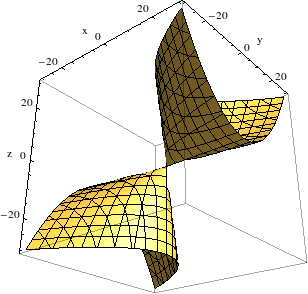
\includegraphics[scale=0.5,keepaspectratio=true]{./scone.png} \\
    The elliptic cone $y^2=xz$ in $\R^3.$
\end{figure}
\end{frame}

\begin{frame}{Abstract Toric Varieties}
 

\begin{Example}
Take $\Delta = \{0, \sigma, \sigma'\}$ as shown below:
\begin{figure}[ht]
  \centering
  \begin{tikzpicture}
    \draw [thin, gray,-latex] (0,0) -- (4,0);% Draw x axis
  \draw [thin, gray,-latex] (0,0) -- (-4,0);% Draw x axis
\foreach \x in {-4,-2,0,2,4}{% Two indices running over each
      \foreach \y in {0}{% node on the grid we have drawn 
        \node[draw,circle,inner sep=1pt,fill] at (\x,\y) {};}}
\draw [ultra thick,-latex,blue] (0,0)
        -- (2,0) node [below ]{$e_1$};
\draw [ultra thick,-latex,blue] (0,0)
        -- (-2,0) node [below] {$-e_1$};
\draw [blue] (0,0) node [below]{0};
\draw (-0.7,0.5) node{\scalebox{1.2}{$\sigma'$ }};
\draw (0.9,0.45) node{\scalebox{1.2}{$\sigma$ }};
  \end{tikzpicture}
\end{figure}

We have $\sigma = \sigma^{\V} = \Cone(e_1)$ so $M_{\sigma}$ is generated by $e_1$ so $\C[M_{\sigma}] = \C[X].$ Similarly, $\sigma' = (\sigma')^{\V} =\Cone(-e_1)$ so $M_{\sigma'}$ is generated by $-e_1$ and $\C[M_{\sigma'}]=\C[X^{-1}].$ We know $\C[M_{0}] = \C[X,X^{-1}].$ 
\end{Example}
\end{frame}

\begin{frame}Both $U_{\sigma}$ and $U_{\sigma'}$ are copies of $\C$ and $X(\Delta)$ is obtained by gluing the images of the embeddings $$ \imath : U_0 = \Spec \C[X,X^{-1}] \to U_{\sigma} = \Spec \C[X] $$ $$ \ \imath': U_{0} = \Spec \C[X,X^{-1}] \to U_{\sigma'} = \Spec \C[X^{-1}] . $$ Therefore we have $$X(\Delta) = \frac{ \C \bigsqcup \C}{ (a \sim a^{-1})_{a\neq 0} }.$$ 

Recall $\Proj^1(\C) = \{ [x:1] \ | \ x\in \C \} \cup \{ [1:x] \ | \ x\in \C \}$ where the overlap is glued via the identification $[a:1] = [1:a^{-1}]$ for all $a\neq 0.$ So $X(\Delta) = \Proj^1(\C).$ 
\end{frame}

\begin{frame}
 Generally, $\Proj^n(\C)= X(\Delta)$ where $\Delta = \{ \Cone(E) | E\subset \{ e_1,\ldots, e_n, -(e_1+\ldots+e_n) \} \}.$ 
    \begin{figure}[ht]
  \centering
  \begin{tikzpicture}
    \draw [thin, gray,-latex] (-1.2,0) -- (1.2,0);% Draw x axis
    \draw [thin, gray,-latex] (0,-1.2) -- (0,1.2);% Draw y axis
    \clip (-1.25,-1.25) rectangle (1.25cm,1.25cm); 
    \draw[style=help lines,dashed] (-4,-4) grid[step=1cm] (4,4);
    \foreach \x in {-5,-4,...,5}{% Two indices running over each
      \foreach \y in {-5,-4,...,5}{% node on the grid we have drawn 
        \node[draw,circle,inner sep=1pt,fill] at (\x,\y) {};}}
    \draw [ultra thick,-latex,blue] (0,0)
        -- (0,1) node [below left] {$e_2$};
    \draw [ultra thick,-latex,blue] (0,0)
        -- (1,0) node [below left] {$e_1$};
\draw [ultra thick,-latex,blue] (0,0)
        -- (-1,-1);
    \filldraw[fill=gray, fill opacity=0.20, draw=black] (0,0) -- (0,1.2) -- (1.2,1.2) -- (1.2, 0) -- (0,0);
    \filldraw[fill=gray, fill opacity=0.60, draw=black] (0,0) -- (1.2,0) -- (1.2,-1.2) -- (-1.2, -1.2) -- (0,0);
    \filldraw[fill=gray, fill opacity=0.35, draw=black] (0,0) -- (0,1.2) -- (-1.2,1.2) -- (-1.2, -1.2) -- (0,0);
    \draw (0.5,0.5) node{\scalebox{1.2}{$\sigma_1$ }};
\draw (-0.4,0.5) node{\scalebox{1.2}{$\sigma_2$ }};
\draw (0.6,-0.5) node{\scalebox{1.2}{$\sigma_3$ }};
  \end{tikzpicture}
  \label{figure:lattice9}
\end{figure}

More examples: 

\begin{itemize}
 \item $Y^{n+1}=XZ$ (Rational singularity of type $A_n$)
\item $WZ = XY $ (Cone over a quadric)
 \item $Y^2=X^3$ (Plane curve with a cusp)
 \item $V(WY-X^2, WZ-XY,XZ-Y^2)\subset \Proj^3(\C)$ (Twisted cubic curve in $\Proj^3(\C).$)
\end{itemize}
$\C^n,$ blow ups of projective space, Hirzebruch surfaces, rational normal scrolls ...
\end{frame}


\end{document}
